\documentclass{standalone}
    \usepackage{tikz}
    \usepackage{amsfonts}
    \usepackage{cmbright}
    \begin{document}
    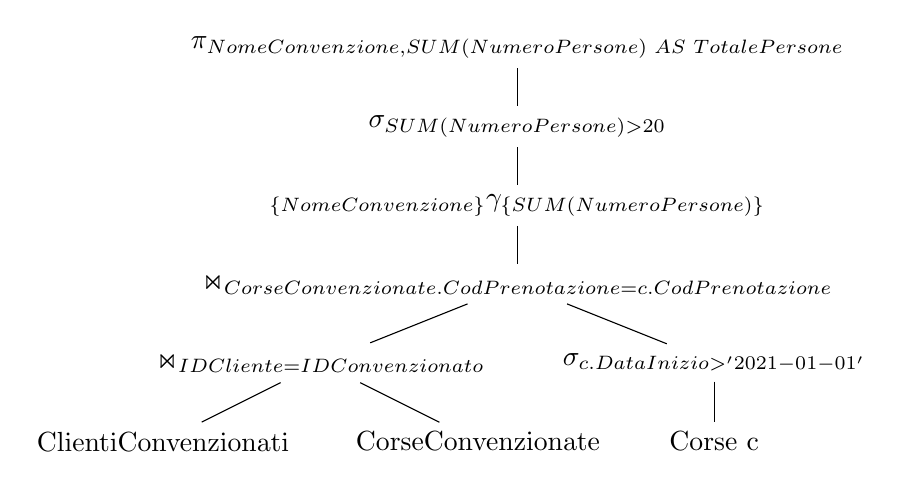
\begin{tikzpicture}
    \newcommand{\lpar}{(}
    \newcommand{\rpar}{)}\node (node) at (0, -1){$\pi_{NomeConvenzione,SUM(NumeroPersone) \,\,AS\,\,TotalePersone}$};
\node (node0) at (0, -2){$\sigma_{SUM \lpar NumeroPersone\rpar > 20
}$};
\node (node00) at (0, -3){$_{\{NomeConvenzione\}}\gamma_{\{SUM(NumeroPersone)\}}$};
\node (node000) at (0, -4){$\Join_{CorseConvenzionate.CodPrenotazione = c.CodPrenotazione
                }$};
\node (node0000) at (-2.5, -5){$\Join_{ IDCliente = IDConvenzionato
                    }$};
\node (node00000) at (-4.5, -6){     ClientiConvenzionati};
\node (node00001) at (-0.5, -6){CorseConvenzionate
                    };
\node (node0001) at (2.5, -5){$\sigma_{ c.DataInizio > '2021-01-01'
                    }$};
\node (node00010) at (2.5, -6){Corse c
                    };
\draw(node) -- (node0);
\draw(node0) -- (node00);
\draw(node00) -- (node000);
\draw(node000) -- (node0000);
\draw(node000) -- (node0001);
\draw(node0000) -- (node00000);
\draw(node0000) -- (node00001);
\draw(node0001) -- (node00010);
\end{tikzpicture}

\end{document}
